% Options for packages loaded elsewhere
\PassOptionsToPackage{unicode}{hyperref}

% Set document class options
\documentclass[webpdf,large,traditional,namedate]{oup-authoring-template}

% one column
\onecolumn

%\usepackage{showframe}

% line numbers

% use upquote if available, for straight quotes in verbatim environments
\IfFileExists{upquote.sty}{\usepackage{upquote}}{}

% From Pandoc template for its feature
\usepackage{xcolor}
\usepackage{hyperref}

\hypersetup{
  pdftitle={Examining Notions of Racism in STEM},
  pdfkeywords={keyword1, keyword2, keyword3},
  breaklinks=true,
  bookmarks=true,
  hidelinks,
  pdfcreator={LaTeX via pandoc}}


% Pandoc syntax highlighting
\usepackage{color}
\usepackage{fancyvrb}
\newcommand{\VerbBar}{|}
\newcommand{\VERB}{\Verb[commandchars=\\\{\}]}
\DefineVerbatimEnvironment{Highlighting}{Verbatim}{commandchars=\\\{\}}
% Add ',fontsize=\small' for more characters per line
\usepackage{framed}
\definecolor{shadecolor}{RGB}{248,248,248}
\newenvironment{Shaded}{\begin{snugshade}}{\end{snugshade}}
\newcommand{\AlertTok}[1]{\textcolor[rgb]{0.94,0.16,0.16}{#1}}
\newcommand{\AnnotationTok}[1]{\textcolor[rgb]{0.56,0.35,0.01}{\textbf{\textit{#1}}}}
\newcommand{\AttributeTok}[1]{\textcolor[rgb]{0.13,0.29,0.53}{#1}}
\newcommand{\BaseNTok}[1]{\textcolor[rgb]{0.00,0.00,0.81}{#1}}
\newcommand{\BuiltInTok}[1]{#1}
\newcommand{\CharTok}[1]{\textcolor[rgb]{0.31,0.60,0.02}{#1}}
\newcommand{\CommentTok}[1]{\textcolor[rgb]{0.56,0.35,0.01}{\textit{#1}}}
\newcommand{\CommentVarTok}[1]{\textcolor[rgb]{0.56,0.35,0.01}{\textbf{\textit{#1}}}}
\newcommand{\ConstantTok}[1]{\textcolor[rgb]{0.56,0.35,0.01}{#1}}
\newcommand{\ControlFlowTok}[1]{\textcolor[rgb]{0.13,0.29,0.53}{\textbf{#1}}}
\newcommand{\DataTypeTok}[1]{\textcolor[rgb]{0.13,0.29,0.53}{#1}}
\newcommand{\DecValTok}[1]{\textcolor[rgb]{0.00,0.00,0.81}{#1}}
\newcommand{\DocumentationTok}[1]{\textcolor[rgb]{0.56,0.35,0.01}{\textbf{\textit{#1}}}}
\newcommand{\ErrorTok}[1]{\textcolor[rgb]{0.64,0.00,0.00}{\textbf{#1}}}
\newcommand{\ExtensionTok}[1]{#1}
\newcommand{\FloatTok}[1]{\textcolor[rgb]{0.00,0.00,0.81}{#1}}
\newcommand{\FunctionTok}[1]{\textcolor[rgb]{0.13,0.29,0.53}{\textbf{#1}}}
\newcommand{\ImportTok}[1]{#1}
\newcommand{\InformationTok}[1]{\textcolor[rgb]{0.56,0.35,0.01}{\textbf{\textit{#1}}}}
\newcommand{\KeywordTok}[1]{\textcolor[rgb]{0.13,0.29,0.53}{\textbf{#1}}}
\newcommand{\NormalTok}[1]{#1}
\newcommand{\OperatorTok}[1]{\textcolor[rgb]{0.81,0.36,0.00}{\textbf{#1}}}
\newcommand{\OtherTok}[1]{\textcolor[rgb]{0.56,0.35,0.01}{#1}}
\newcommand{\PreprocessorTok}[1]{\textcolor[rgb]{0.56,0.35,0.01}{\textit{#1}}}
\newcommand{\RegionMarkerTok}[1]{#1}
\newcommand{\SpecialCharTok}[1]{\textcolor[rgb]{0.81,0.36,0.00}{\textbf{#1}}}
\newcommand{\SpecialStringTok}[1]{\textcolor[rgb]{0.31,0.60,0.02}{#1}}
\newcommand{\StringTok}[1]{\textcolor[rgb]{0.31,0.60,0.02}{#1}}
\newcommand{\VariableTok}[1]{\textcolor[rgb]{0.00,0.00,0.00}{#1}}
\newcommand{\VerbatimStringTok}[1]{\textcolor[rgb]{0.31,0.60,0.02}{#1}}
\newcommand{\WarningTok}[1]{\textcolor[rgb]{0.56,0.35,0.01}{\textbf{\textit{#1}}}}

% tightlist command for lists without linebreak
\providecommand{\tightlist}{%
  \setlength{\itemsep}{0pt}\setlength{\parskip}{0pt}}




% Counters for addresses and footnotes
\newcounter{correspcnt} % For author footnotes
\renewcommand*{\thecorrespcnt}{\fnsymbol{correspcnt}}
\newcounter{addrcnt} % For author addresses

% Macros for dealing with affiliations, footnotes, etc.
\makeatletter

\def\MyNewLabel#1#2#3{\expandafter\gdef\csname #1@#2\endcsname{#3}}

\def\MyRef#1#2{\@ifundefined{#1@#2}{???}{\csname #1@#2\endcsname}}

\newcommand*\ifcounter[1]{%
  \ifcsname c@#1\endcsname
    \expandafter\@firstoftwo
  \else
    \expandafter\@secondoftwo
  \fi
}

\newcommand*\addrlblbycode[1]{%
  \ifcounter{ADDRLBL@#1}
    {}
    {\refstepcounter{addrcnt}\newcounter{ADDRLBL@#1}\setcounter{ADDRLBL@#1}{\value{addrcnt}}}%
    \arabic{ADDRLBL@#1}%
}

\newcommand*\addrbycode[1]{%
  \ifcounter{ADDR@#1}
    {}
    {\newcounter{ADDR@#1}%
     \address[\addrlblbycode{#1}]{\MyRef{ADDRTXT}{#1}}}%
}

\newcommand*\corresplblbycode[1]{%
  \ifcounter{CORRESPLBL@#1}
    {}
    {\refstepcounter{correspcnt}\newcounter{CORRESPLBL@#1}\setcounter{CORRESPLBL@#1}{\value{correspcnt}}}%
    \fnsymbol{CORRESPLBL@#1}%
}

\newcommand*\correspbycode[1]{%
  \ifcounter{CORRESP@#1}
    {}
    {\newcounter{CORRESP@#1}%
     \corresp[\corresplblbycode{#1}]{\MyRef{CORRESPTXT}{#1}}}%
}

\makeatother

% Add missing \city command mentioned in documentation but absent from cls
\providecommand\city[1]{#1}

% Create labels for Addresses if the are given in Elsevier format

% Create labels for Footnotes if they are given in Elsevier format

% Pandoc header-include feature
\usepackage{booktabs}

\begin{document}

\journaltitle{Journal Title Here}
\DOI{DOI HERE}
\copyrightyear{YYYY}
\pubyear{YYYY}
\access{Advance Access Publication Date: Day Month Year}
\appnotes{Paper}

\firstpage{1}



\title[]{Examining Notions of Racism in STEM}

\newcounter{thisauthcorresp} % For storage if author is corresponding author
\newcounter{thisauththanks} % For storage if author has thanks



% Add author mark

\received{Date}{0}{Year}
\revised{Date}{0}{Year}
\accepted{Date}{0}{Year}

%\editor{Associate Editor: Name}

\abstract{
This is the first paragraph of the abstract. It has several sentences
making it go over several lines. For this it needs to have a lot of
text.\\
This is the second paragraph.\\
\textbf{Motivation:} You can also have some paragraphs start with bold
face.}

\keywords{keyword1; keyword2; keyword3}


\maketitle


\hypertarget{introduction}{%
\section{Introduction}\label{introduction}}

This template is based on the generic OUP authoring template available
on CTAN under
\href{https://www.ctan.org/pkg/oup-authoring-template}{oup-authoring-template}.
The CTAN template includes LaTeX documentation and a sample LaTeX
document that provide far more details regarding the full functionality
of the format. Here, only the basic functioning of the Rmarkdown
adaptation of the format is demonstrated.

\hypertarget{a-subsection}{%
\subsection{A subsection}\label{a-subsection}}

A numbered list:

\begin{enumerate}
\def\labelenumi{\arabic{enumi})}
\tightlist
\item
  First point
\item
  Second point

  \begin{itemize}
  \tightlist
  \item
    Subpoint
  \end{itemize}
\end{enumerate}

A bullet list:

\begin{itemize}
\tightlist
\item
  First point
\item
  Second point
\end{itemize}

\hypertarget{notes}{%
\subsection{Notes}\label{notes}}

\begin{itemize}
\tightlist
\item
  Extra white space in document will tend to disappear as text is filled
  in.
\item
  Code blocks tend to generate lots of empty white space when
  \texttt{echo=TRUE} for some reason.
\end{itemize}

\hypertarget{literature-citations}{%
\section{Literature citations}\label{literature-citations}}

By default, citations are handled by \texttt{natbib} using a numeric
citation format. To use name-date citations, sets
\texttt{namedate:\ TRUE} in the YAML header.

Here are two sample references:

\begin{itemize}
\tightlist
\item
  \textbf{author (year) example:} \citet{horvath2018dna} showed some
  really cool things. Only seems to work properly if
  \texttt{namedate:\ TRUE}.
\item
  \textbf{(author year) example:} This is a well known result
  \citep{ji20123d}.
\end{itemize}

The bibliography will appear at the end of the document.

Though not normally available in the OUP LaTeX format,
\href{https://www.zotero.org/styles}{CSL style files} can also be used
with the Rmarkdown adaptation by setting in the YAML header
\texttt{citation\_package:\ "default"} and defining the \texttt{csl}
element to be the path towards the style file.

\hypertarget{equations}{%
\section{Equations}\label{equations}}

An equation without a label for cross-referencing:

\[
E=mc^2
\]

An inline equation: \(y=ax+b\)

An equation with a label for cross-referencing:

\begin{equation}\label{eq:eq1}
\int^{r_2}_0 F(r,\varphi){\rm d}r\,{\rm d}\varphi = 1
\end{equation}

This equation can be referenced as follows: Eq. \ref{eq:eq1}

\hypertarget{inserting-r-figures}{%
\section{Inserting R figures}\label{inserting-r-figures}}

The code below creates a figure. The code is included in the output
because \texttt{echo=TRUE}.

\begin{Shaded}
\begin{Highlighting}[]
\FunctionTok{plot}\NormalTok{(}\DecValTok{1}\SpecialCharTok{:}\DecValTok{10}\NormalTok{,}\AttributeTok{main=}\StringTok{"Some data"}\NormalTok{,}\AttributeTok{xlab=}\StringTok{"Distance (cm)"}\NormalTok{,}
     \AttributeTok{ylab=}\StringTok{"Time (hours)"}\NormalTok{)}
\end{Highlighting}
\end{Shaded}

\begin{figure}[th]
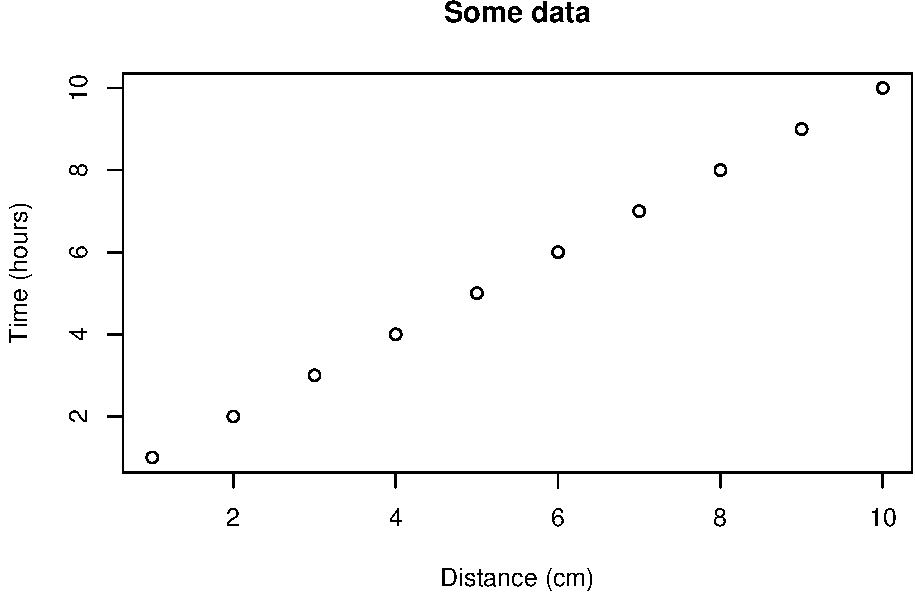
\includegraphics[width=1\linewidth]{Examining-Notions-of-Racism-in-STEM_files/figure-latex/fig1-1} \caption{This is the first figure.}\label{fig:fig1}
\end{figure}

You can reference this figure as follows: Fig. \ref{fig:fig1}.

\hypertarget{figures-spanning-two-columns}{%
\subsection{Figures spanning
two-columns}\label{figures-spanning-two-columns}}

Figures can span two columns be setting \texttt{fig.env="figure*"}.

\begin{figure*}[th]
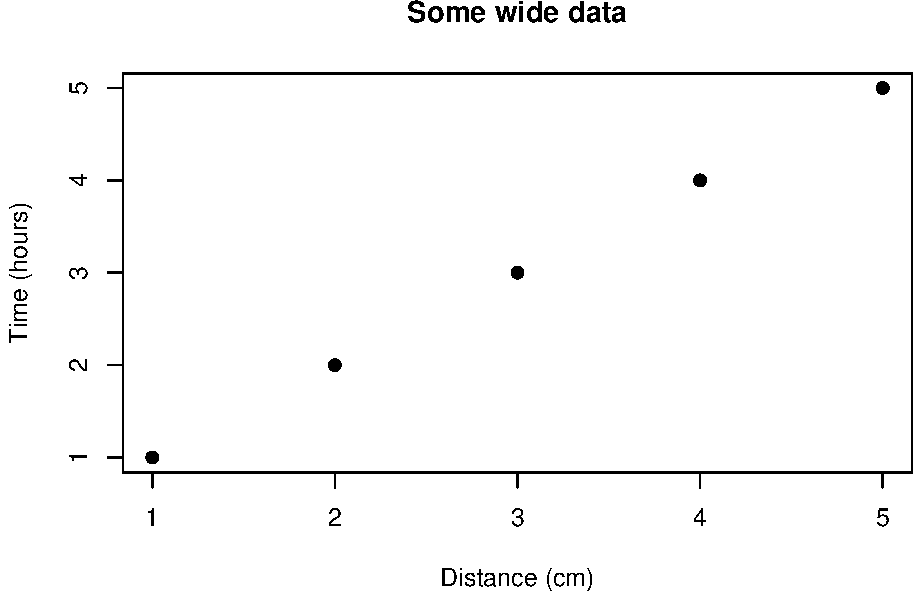
\includegraphics[width=1\linewidth]{Examining-Notions-of-Racism-in-STEM_files/figure-latex/fig2-1} \caption{This is a wide figure.}\label{fig:fig2}
\end{figure*}

Reference to second figure: Fig. \ref{fig:fig2}

\hypertarget{tables}{%
\section{Tables}\label{tables}}

\hypertarget{generate-a-table-using-xtable}{%
\subsection{\texorpdfstring{Generate a table using
\texttt{xtable}}{Generate a table using xtable}}\label{generate-a-table-using-xtable}}

\begin{Shaded}
\begin{Highlighting}[]
\NormalTok{df }\OtherTok{=} \FunctionTok{data.frame}\NormalTok{(}\AttributeTok{ID=}\DecValTok{1}\SpecialCharTok{:}\DecValTok{3}\NormalTok{,}\AttributeTok{code=}\NormalTok{letters[}\DecValTok{1}\SpecialCharTok{:}\DecValTok{3}\NormalTok{])}

\CommentTok{\# Creates tables that follow OUP guidelines }
\CommentTok{\# using xtable}
\FunctionTok{library}\NormalTok{(xtable) }
\FunctionTok{print}\NormalTok{(}\FunctionTok{xtable}\NormalTok{(df,}\AttributeTok{caption=}\StringTok{"This is a xtable table."}\NormalTok{,}
             \AttributeTok{label=}\StringTok{"tab:tab1"}\NormalTok{),}
      \AttributeTok{comment=}\ConstantTok{FALSE}\NormalTok{,}\AttributeTok{caption.placement=}\StringTok{"top"}\NormalTok{)}
\end{Highlighting}
\end{Shaded}

\begin{table}[ht]
\centering
\caption{This is a xtable table.} 
\label{tab:tab1}
\begin{tabular}{rrl}
  \hline
 & ID & code \\ 
  \hline
1 &   1 & a \\ 
  2 &   2 & b \\ 
  3 &   3 & c \\ 
   \hline
\end{tabular}
\end{table}

You can reference this table as follows: Table \ref{tab:tab1}.

\hypertarget{generate-a-table-using-kable}{%
\subsection{\texorpdfstring{Generate a table using
\texttt{kable}}{Generate a table using kable}}\label{generate-a-table-using-kable}}

\begin{Shaded}
\begin{Highlighting}[]
\NormalTok{df }\OtherTok{=} \FunctionTok{data.frame}\NormalTok{(}\AttributeTok{ID=}\DecValTok{1}\SpecialCharTok{:}\DecValTok{3}\NormalTok{,}\AttributeTok{code=}\NormalTok{letters[}\DecValTok{1}\SpecialCharTok{:}\DecValTok{3}\NormalTok{])}

\CommentTok{\# kable can alse be used for creating tables}
\NormalTok{knitr}\SpecialCharTok{::}\FunctionTok{kable}\NormalTok{(df,}\AttributeTok{caption=}\StringTok{"This is a kable table."}\NormalTok{,}
             \AttributeTok{booktabs=}\ConstantTok{TRUE}\NormalTok{,}\AttributeTok{label=}\StringTok{"tab2"}\NormalTok{)}
\end{Highlighting}
\end{Shaded}

\begin{table}

\caption{\label{tab:tab2}This is a kable table.}
\centering
\begin{tabular}[t]{rl}
\toprule
ID & code\\
\midrule
1 & a\\
2 & b\\
3 & c\\
\bottomrule
\end{tabular}
\end{table}

You can reference this table as follows: Table \ref{tab:tab2}.

\hypertarget{table-spanning-two-columns}{%
\subsection{Table spanning two
columns}\label{table-spanning-two-columns}}

Tables can span two columns be setting \texttt{table.envir\ =\ "table*"}
in \texttt{knitr::kable}.

\begin{Shaded}
\begin{Highlighting}[]
\NormalTok{df }\OtherTok{=} \FunctionTok{data.frame}\NormalTok{(}\AttributeTok{ID=}\DecValTok{1}\SpecialCharTok{:}\DecValTok{3}\NormalTok{,}\AttributeTok{code1=}\NormalTok{letters[}\DecValTok{1}\SpecialCharTok{:}\DecValTok{3}\NormalTok{],}
                \AttributeTok{code2=}\NormalTok{letters[}\DecValTok{4}\SpecialCharTok{:}\DecValTok{6}\NormalTok{],}
                \AttributeTok{code3=}\NormalTok{letters[}\DecValTok{7}\SpecialCharTok{:}\DecValTok{9}\NormalTok{],}
                \AttributeTok{code4=}\NormalTok{letters[}\DecValTok{10}\SpecialCharTok{:}\DecValTok{12}\NormalTok{],}
                \AttributeTok{code5=}\NormalTok{letters[}\DecValTok{13}\SpecialCharTok{:}\DecValTok{15}\NormalTok{])}

\CommentTok{\# kable can alse be used for creating tables}
\NormalTok{knitr}\SpecialCharTok{::}\FunctionTok{kable}\NormalTok{(df,}\AttributeTok{caption=}\StringTok{"This is a wide kable table."}\NormalTok{,}
             \CommentTok{\#format="latex",}
             \AttributeTok{table.envir=}\StringTok{"table*"}\NormalTok{,}
             \AttributeTok{booktabs=}\ConstantTok{TRUE}\NormalTok{,}\AttributeTok{label=}\StringTok{"tab3"}\NormalTok{)}
\end{Highlighting}
\end{Shaded}

\begin{table*}

\caption{\label{tab:tab3}This is a wide kable table.}
\centering
\begin{tabular}[t]{rlllll}
\toprule
ID & code1 & code2 & code3 & code4 & code5\\
\midrule
1 & a & d & g & j & m\\
2 & b & e & h & k & n\\
3 & c & f & i & l & o\\
\bottomrule
\end{tabular}
\end{table*}

\hypertarget{cross-referencing-sections}{%
\section{Cross-referencing sections}\label{cross-referencing-sections}}

You can cross-reference sections and subsections as follows: Section
\ref{literature-citations} and Section \ref{a-subsection}.

\textbf{\emph{Note:}} the last section in the document will be used as
the section title for the bibliography.

For more portable and flexible referencing of sections, equations,
figures and tables, use
\href{https://github.com/rstudio/bookdown}{\texttt{bookdown::pdf\_document2}}
with YAML header option \texttt{base\_format:\ rticles::oup\_article}.

\hypertarget{appendices}{%
\section*{Appendices}\label{appendices}}
\addcontentsline{toc}{section}{Appendices}

\begin{appendices}

\hypertarget{section-title-of-first-appendix}{%
\section{Section title of first
appendix}\label{section-title-of-first-appendix}}

blabla

\hypertarget{subsection-title-of-first-appendix}{%
\subsection{Subsection title of first
appendix}\label{subsection-title-of-first-appendix}}

and so on\ldots.

\end{appendices}

\section{Competing interests}

There are no competing interest.


\renewcommand\refname{References}

\bibliographystyle{abbrvnat}
\bibliography{mybibfile.bib}

%% Author bio-pics with images


\end{document}
